\documentclass[tikz,border=8pt]{standalone}
\usepackage{amsmath,amssymb}
\usetikzlibrary{arrows.meta,automata,positioning,quotes}
\begin{document}
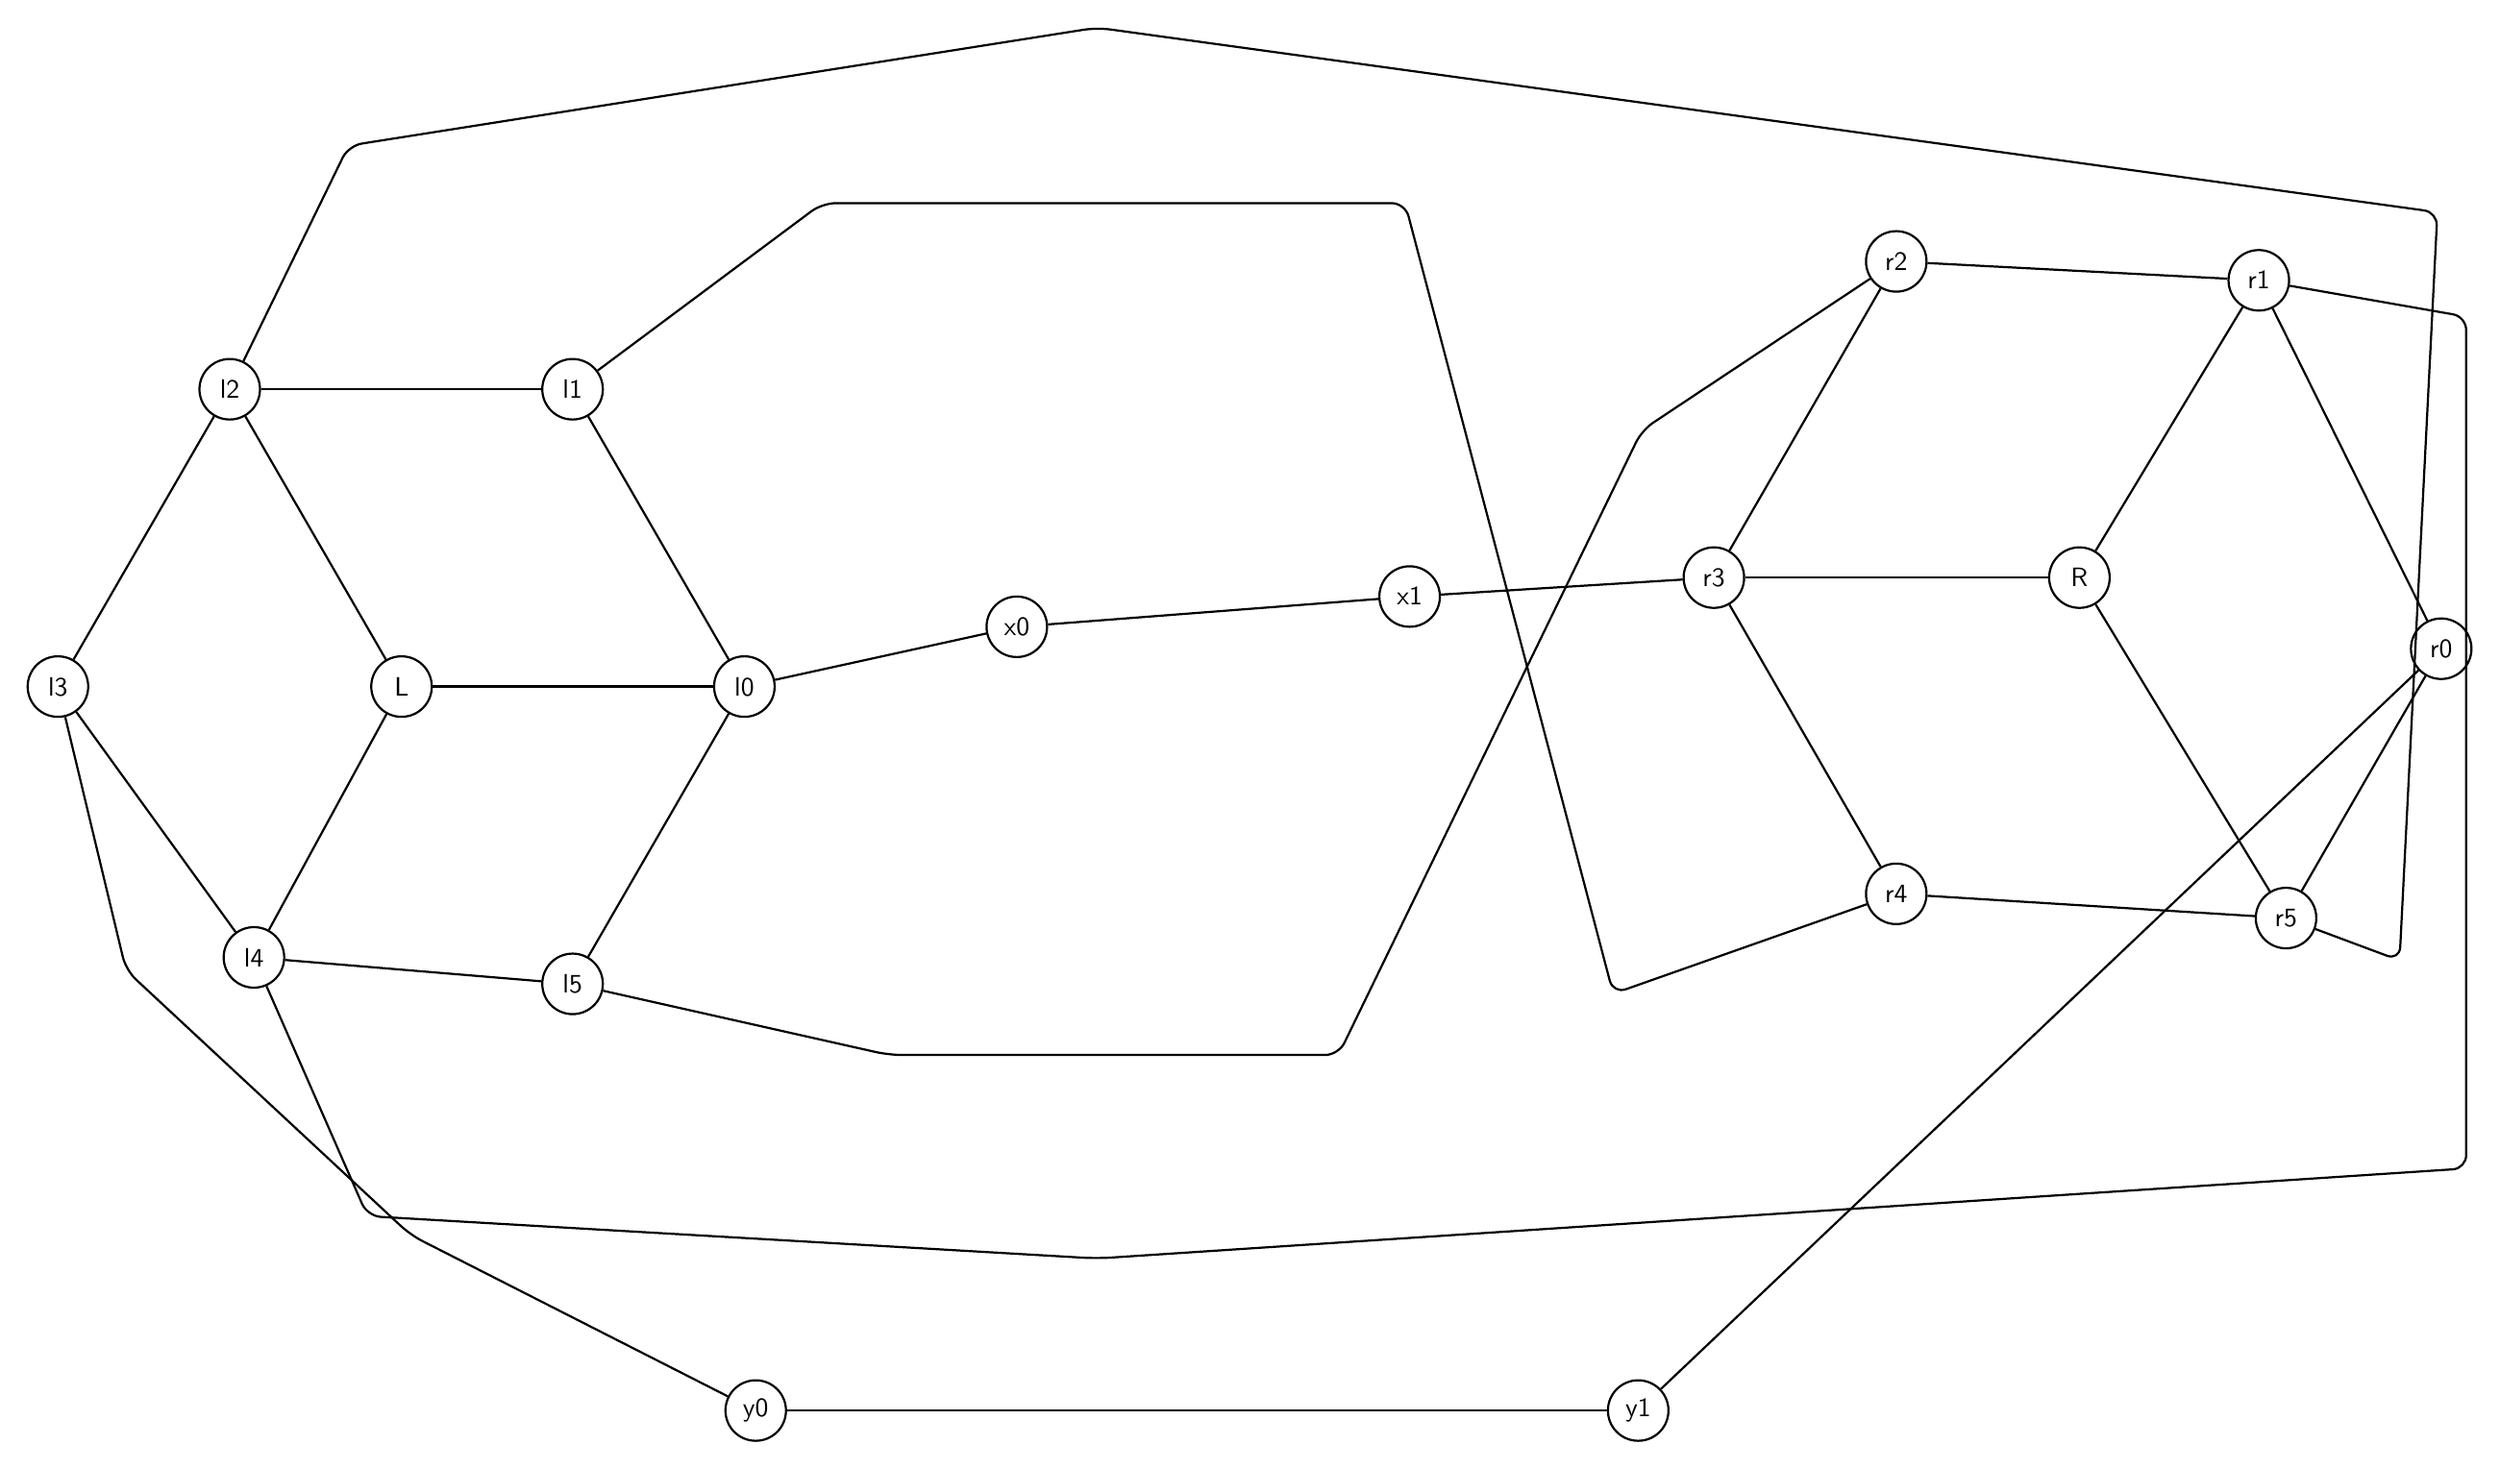
\begin{tikzpicture}[x=1cm,y=1cm]
\tikzset{
  graphnode/.style={circle,draw,thick,minimum size=8mm,inner sep=1pt,font=\sffamily},
  directed/.style={-{Stealth[length=2.4mm]},thick},
  undirected/.style={thick}
}
\node[graphnode] (n_L) at (-11.28,0.25) {L};
\node[graphnode] (n_l0) at (-6.75,0.25) {l0};
\node[graphnode] (n_l1) at (-9.02,4.18) {l1};
\node[graphnode] (n_l2) at (-13.55,4.18) {l2};
\node[graphnode] (n_l3) at (-15.82,0.25) {l3};
\node[graphnode] (n_l4) at (-13.23,-3.33) {l4};
\node[graphnode] (n_l5) at (-9.02,-3.68) {l5};
\node[graphnode] (n_R) at (10.89,1.69) {R};
\node[graphnode] (n_r0) at (15.67,0.75) {r0};
\node[graphnode] (n_r1) at (13.26,5.62) {r1};
\node[graphnode] (n_r2) at (8.47,5.87) {r2};
\node[graphnode] (n_r3) at (6.06,1.69) {r3};
\node[graphnode] (n_r4) at (8.47,-2.49) {r4};
\node[graphnode] (n_r5) at (13.62,-2.81) {r5};
\node[graphnode] (n_x0) at (-3.15,1.04) {x0};
\node[graphnode] (n_x1) at (2.04,1.44) {x1};
\node[graphnode] (n_y0) at (-6.60,-9.32) {y0};
\node[graphnode] (n_y1) at (5.06,-9.32) {y1};
\draw[undirected] (n_l0) -- (n_l1);
\draw[undirected] (n_l1) -- (n_l2);
\draw[undirected] (n_l2) -- (n_l3);
\draw[undirected] (n_l3) -- (n_l4);
\draw[undirected] (n_l4) -- (n_l5);
\draw[undirected] (n_l5) -- (n_l0);
\draw[undirected] (n_L) -- (n_l0);
\draw[undirected] (n_L) -- (n_l2);
\draw[undirected] (n_L) -- (n_l4);
\draw[undirected] (n_r0) -- (n_r1);
\draw[undirected] (n_r1) -- (n_r2);
\draw[undirected] (n_r2) -- (n_r3);
\draw[undirected] (n_r3) -- (n_r4);
\draw[undirected] (n_r4) -- (n_r5);
\draw[undirected] (n_r5) -- (n_r0);
\draw[undirected] (n_R) -- (n_r1);
\draw[undirected] (n_R) -- (n_r3);
\draw[undirected] (n_R) -- (n_r5);
\draw[undirected] (n_l0) -- (n_x0);
\draw[undirected] (n_x0) -- (n_x1);
\draw[undirected] (n_x1) -- (n_r3);
\draw[undirected,rounded corners=5pt] (n_l3) -- (-14.92,-3.50) -- (-11.16,-7.00) -- (n_y0);
\draw[undirected] (n_y0) -- (n_y1);
\draw[undirected] (n_y1) -- (n_r0);
\draw[undirected,rounded corners=5pt] (n_l1) -- (-5.72,6.64) -- (1.98,6.64) -- (4.73,-3.81) -- (n_r4);
\draw[undirected,rounded corners=5pt] (n_l2) -- (-11.98,7.40) -- (-2.09,8.96) -- (15.62,6.52) -- (15.12,-3.37) -- (n_r5);
\draw[undirected,rounded corners=5pt] (n_l4) -- (-11.73,-6.75) -- (-2.09,-7.31) -- (16.00,-6.12) -- (16.00,5.14) -- (n_r1);
\draw[undirected,rounded corners=5pt] (n_l5) -- (-4.84,-4.62) -- (1.10,-4.62) -- (5.11,3.64) -- (n_r2);
\end{tikzpicture}
\end{document}
